% !TeX root=../main.tex
\chapter{نظریه گراف}
%\thispagestyle{empty} 
\section{پیشگفتار} 
امروزه نظریه گراف و الگوریتم های آن نقش مهمی را در بسیاری از علوم بازی میکند، بسیاری از مفاهیم پیچیده از علوم فیزیک و شیمی گرفته تا علوم کامپیوتر توسط نظریه گراف توصیف میشود.
در این فصل علاوه بر مرور مختصر بر مفاهیم گراف، به الگوریتم هایی که در یافتن پاسخ خودکار مدار به ما یاری می رسانند پرداخته میشود.

\section{گراف}
گراف یک جفت مرتب
\footnote{
	گراف میتواند جهت دار یا بدون جهت باشد اگر گراف یاد شده بی جهت باشد استفاده از عبارت 
	«جفت» کافی است
	در غیر این صورت بایستی عبارت «جفت مرتب» را به کار برد. 
}
 به صورت
 $G = (V,E)$
 است به گونه ای که
  \lr{V}
 مجموعه ای از راس های گراف و
 $ E \subseteq \{(x,y)|(x,y) \in V^2 \}  $
 مجموعه یال های گراف است.
 با توجه به گستردگی نظریه گراف انواع زیادی از مفاهیم و الگوریتم ها درباره گراف موجود است
 ما در این فصل به توضیح آنچه که در پروژه استفاده شده بسنده خواهیم کرد.
\section{دور های ساده گراف}
اگر در یک گراف مجموعه ای از یال ها از یک راس مشخص شروع شده و با همان راس یاد شده خاتمه یابد
به آن مجموعه یک دور میگویم.
به دوری یک دور ساده
\LTRfootnote{simple cycle }
 گوییم هر آنگاه به جز راس نخستین و پایانی هیچ راس تکراری دیگری موجود نباشد یا به
 عبارت دیگر نتوان دور را به دور های کوچکتری شکست.
 
 به عنوان مثال در شکل
 \ref{fig:fig1} 
 دور
 \lr{ABDCA}
 یک دور ساده نیست چرا که میتواند به دو دور ساده
  \lr{ABCA}
  و
   \lr{BDCB}
   شکسته شود.
 
 \begin{figure}[ht]
 	\centerline{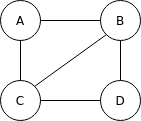
\includegraphics[width=5cm]{fig1}}
 	\caption{یک گراف بدون جهت شامل دو دور ساده}
 	\label{fig:fig1}
 \end{figure}
\subsection{پیدا کردن دور های ساده گراف}
پیدا کردن تمامی دور های ساده گراف از آن جهت برای ما اهمیت دارد که در مدل نهایی هر دور ساده
باعث یافتن یکی از
\LR{KVL}
موجود در مدار میشود.

برای یافتن مجموعه دور های ساده موجود در گراف ابتدا نیاز به یافتن درخت پوشای کمینه
\LTRfootnote{minimum spanning tree}
گراف یاد شده داریم، برای اینکار الگوریتم های زیادی از جمله الگوریتم کراسکال
\LTRfootnote{kruskal}
و الگوریتم پریم
\LTRfootnote{prim}
که در قسمت های
\ref{kruskal}
و
\ref{prim}
آمده است
طراحی شده اند، البته در پروژه حاضر از کتابخانه
\LR{networkx}
پایتون برای پیاده سازی استفاده شده است.

میتوان اثبات کرد که اگر یکی از یال های حذف شده را به درخت پوشای کمینه بیفزایم 
یک و تنها یک دور ساده ایجاد میشود که ما با الگوریتم
\LR{DFS}
که در قسمت
\ref{dfs}
آمده است
\LTRfootnote{depth first search}
آن دور را می یابیم
، سپس با افزودن تمامی یال ها به صورت تک به تک تمامی دور های ساده یافت میشود.

به عنوان نمونه اگه گراف شکل
\ref{fig:fig1}
ورودی ما باشد درخت پوشای کمینه ما شکل
\ref{fig:fig2}
خواهد بود که دارای دو یال قطع شده
\lr{AB}
و
\lr{BD}
است.که با نقطه چین نمایش داده شده اند.
با اضافه کردن یال های قطع شده به صورت تک به تک دو گراف شکل
\ref{fig:fig3}
پدید می آیند که هر کدام دارای دارای یک دور ساده هستند سپس همانطور که یاد شد
با الگوریتم
\lr{DFS}
دور های مورد نظر را می یابیم.
الگوریتم توضیح داده شده به صورت شبه کد در قسمت
\ref{simpcyc}
آمده است.
\cite{Dorfler18}
\begin{figure}[ht]
	\centerline{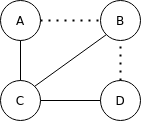
\includegraphics[width=5cm]{fig2}}
	\caption{درخت پوشای کمینه شکل
	\ref{fig:fig1} }
	\label{fig:fig2}
\end{figure}

\begin{figure}[ht]
	\centerline{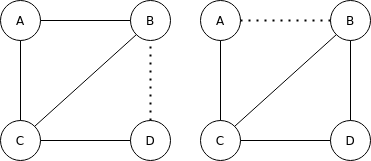
\includegraphics[width=9cm]{fig3}}
	\caption{دو گراف تک ساده دور شکل
		\ref{fig:fig1} }
	\label{fig:fig3}
\end{figure}
\begin{algorithm}[ht]
	\onehalfspacing
	\caption{الگوریتم پیدا کردن مجموعه دور های ساده گراف} 
	\label{simpcyc}
	\begin{algorithmic}[1]
		\REQUIRE
		\lr{graph}
		\ENSURE
		\lr{simple cycle entity}
		\STATE 
		\lr{create simple-cycles entity s = \{\}}
		\STATE 
		\lr{mst = kruskal(graph)}
		\STATE 
		\lr{store in stack s = graph - mst}
		\STATE
		\lr{store s.pop() in edge e}
		\STATE
		\lr{create new graph g = mst + e}
		\STATE
		\lr{define cycle c = dfs(g)}
		\STATE
		\lr{add cycle c to entity s }
		\STATE
		\lr{if stack s terminate the program otherwise return to instruction number4 }
	\end{algorithmic}
\end{algorithm}

\begin{algorithm}[ht]
	\onehalfspacing
	\caption{الگوریتم کراسکال} 
	\label{kruskal}
	\begin{algorithmic}[1]
		\REQUIRE
		\lr{graph}
		\ENSURE
		\lr{minimum spaning tree}
		\STATE
	    \lr{A = \{\}}
	    \STATE
	    \lr{For each vertex v in graph:}
	    \STATE
	    \lr{MAKE-SET(v)}
	    \STATE
		\lr{For each edge (u, v) in graph ordered by increasing order by weight(u, v):}
		\STATE
	    \lr{if FIND-SET(u) != FIND-SET(v):}
	    \STATE
	    \lr{A = A union (u, v)}
	    \STATE
	    \lr{UNION(u, v)}
	    \STATE
	    \lr{return A} 
	\end{algorithmic}
\end{algorithm}

\begin{algorithm}[ht]
	\onehalfspacing
	\caption{الگوریتم پریم} 
	\label{prim}
	\begin{algorithmic}[1]
		\REQUIRE
		\lr{graph}
		\ENSURE
		\lr{minimum spaning tree}
		\STATE
		\lr{A = \{\}}
		\STATE
		\lr{U = \{ 1 \}}
		\STATE
		\lr{while (U != V)}
		\STATE
		\lr{let (u, v) be the lowest cost edge such that u in U and v in V - U:}
		\STATE
		\lr{T = T union (u, v)}
		\STATE
		\lr{U = U union v}
				
	\end{algorithmic}
\end{algorithm}

\begin{algorithm}[ht]
	\onehalfspacing
	\caption{الگوریتم 
	\lr{dfs}
} 
	\label{dfs}
	\begin{algorithmic}[1]
		\REQUIRE
		\lr{graph}
		\ENSURE
		\lr{Stack S = \{\}}
		\STATE
		\lr{for each vertex u, set visited[u] = false}
		\STATE
		\lr{push v to S}
		\STATE
		\lr{while (S is not empty) do}
		\STATE
		\lr{u = S.pop()}
		\STATE
		\lr{while (S is not empty) do}
		\STATE
		\lr{if (not visited[u]) then}
		\STATE
		\lr{visited[u] := true}
		\STATE
		\lr{for each unvisited neighbour w of u}
		\STATE
		\lr{S.push(w)}
		
	\end{algorithmic}
\end{algorithm}

\section{جمع بندی}
در این فصل به مفاهیم نظریه گراف پرداخته شد که در فصل بعدی نقش اصلی را در مدل کردن مدار های الکتریکی به شکل انتزاعی بازی میکنند؛همانطور که پیشتر اشاره شد برای به دست آوردن پاسخ مدار ما نیازمند پیدا کردن تمامی قوانین
\lr{kvl}
هستیم، با در نظر گرفتن مدار به صورت گراف این مسئله به شکل یافتن تمامی دور های ساده گراف
در می آید که در الگوریتم
\eqref{simpcyc}
به آن پرداخته شده است.